% SPDX-License-Identifier: CC-BY-NC-SA-4.0
% Repository edition: substantive v0.3 text preserved; licensed under CC BY-NC-SA 4.0.
\documentclass[11pt]{article}

% arXiv-friendly, journal-neutral preprint with compact tables, in-place
% figures, explicit definitions, and a self-contained bibliography.
\usepackage[T1]{fontenc}
\usepackage[utf8]{inputenc}
\usepackage[english]{babel}
\usepackage{lmodern}
\usepackage[a4paper,margin=24mm]{geometry}
\usepackage{microtype}
\usepackage{amsmath,amssymb,amsthm,mathtools,bm}
\usepackage{booktabs}
\usepackage{array}
\usepackage{enumitem}
\usepackage{tikz}
\usetikzlibrary{arrows.meta,positioning,fit,calc}
\usepackage{xurl}
\usepackage[hidelinks]{hyperref}
\usepackage[nameinlink,noabbrev]{cleveref}

\setlength{\parindent}{1.25em}
\setlength{\parskip}{0.15em}
\setlist{nosep,leftmargin=1.6em}
\allowdisplaybreaks[1]
\hypersetup{
  pdftitle={Operational Equivalence under Evolving Future Tests: Quotient Dynamics across Quantum Processes, Control, and Quantum Geometry},
  pdfauthor={Elaina Lynn Amaral},
  pdfsubject={Operational equivalence, predictive state compression, process tensors, relational observables, spin foams, coarse graining, state abstraction},
  pdfkeywords={operational equivalence, predictive state representation, state abstraction, process tensor, quantum reference frame, spin foam, coarse graining, quantum gravity}
}

\newtheorem{definition}{Definition}
\newtheorem{proposition}[definition]{Proposition}
\newtheorem{conjecture}[definition]{Conjecture}
\newtheorem{remark}[definition]{Remark}
\newtheorem{example}[definition]{Example}

\newcommand{\F}{\mathcal F}
\newcommand{\Sspace}{\mathcal S}
\newcommand{\Y}{\mathcal Y}
\newcommand{\Q}{\mathcal Q}
\newcommand{\Res}{\operatorname{Res}}
\newcommand{\Future}{\operatorname{Future}}
\newcommand{\Disc}{\operatorname{Disc}}
\newcommand{\TV}{D_{\mathrm{TV}}}
\newcommand{\Tr}{\operatorname{Tr}}
\newcommand{\im}{\operatorname{im}}
\newcommand{\id}{\mathrm{id}}
\newcommand{\eps}{\varepsilon}

\title{\bfseries Operational Equivalence under Evolving Future Tests:\\
Quotient Dynamics across Quantum Processes, Control, and Quantum Geometry}
\author{Elaina Lynn Amaral\\
\small Independent publisher\\
\small \href{mailto:17bestradiol@proton.me}{\nolinkurl{17bestradiol@proton.me}}}
\date{September 2026\\[1mm]\small Manuscript v0.3}

\begin{document}
\maketitle

\begin{abstract}
A state description is useful only through distinctions that can change future observations, interventions, or decisions. This paper studies the quotient obtained by identifying states or histories that induce the same statistics for a declared family of future tests. Mature versions of this idea occur in causal states, predictive-state representations, Markov decision-process abstractions, operational quantum theory, quantum processes, and quantum reference frames. We isolate the common quotient, prove its minimal sufficiency property, and extend it to operational distinguishability. The main dynamical result treats the test family itself as time dependent: if later tests pull back through state evolution to distinctions already represented by the earlier family, then the physical evolution descends uniquely to an evolution between quotient states. If this condition fails, a later test can reopen a distinction that an earlier quotient erased. For quantum channels the condition is expressed by the Heisenberg adjoint acting on effects, giving a direct structural-state / observable-family duality. We additionally define operational relational nonfactorization: a joint future map is irreducible relative to declared local descriptions when it does not factor through the product of their local future-sufficient quotients. This is a mechanism-neutral criterion and is explicitly weaker than quantum entanglement. We then formulate a future-sufficient coarse-graining criterion for boundary quantum gravity in which prediction preservation and minimal compression are separate obligations, together with composition, refinement consistency, relational covariance, and semiclassical recovery. The quotient and transport results are exact; the relational factorization criterion is exact once the state and test families are declared; the spin-foam application remains a conjectural physical implementation rather than a claimed solution of the continuum problem.
\end{abstract}

\noindent\textbf{Keywords:} operational equivalence; sufficient representation; relational nonfactorization; predictive state; process tensor; state abstraction; relational observable; quantum reference frame; spin foam; coarse graining; quantum gravity.

\section{Introduction}

Physics routinely discards microscopic detail. Statistical mechanics, effective field theory, numerical renormalization, gauge reduction, and state estimation all work because not every difference in a description remains consequential for the questions being asked. Artificial intelligence does the same under different names: state aggregation, predictive representations, bisimulation, latent-state learning, and model reduction attempt to preserve behavior while reducing description. The hard part is not compression itself. It is specifying, without hindsight or hand-waving, which differences may be erased.

A natural answer is operational. Fix a family of admissible future tests. Two current descriptions are equivalent when no test in that family can distinguish their future consequences. The resulting quotient is the coarsest representation that remains sufficient for those tests. This idea is not new in isolation. Blackwell's comparison of statistical experiments already asks when one experiment preserves every decision-relevant consequence available from another~\cite{blackwell1953}. Computational mechanics constructs causal states by grouping pasts with identical conditional futures~\cite{crutchfield1989,shalizi2001}. Predictive-state representations encode dynamical state through predictions of observable experiments~\cite{littman2001,singh2004}. State abstraction and bisimulation in Markov decision processes identify states that preserve reward and transition-relevant behavior~\cite{givan2003,ferns2011}. Information-bottleneck methods explicitly trade representation complexity against predictive information~\cite{tishby1999,creutzig2009,still2012}. In operational quantum theory, indistinguishability of preparations, transformations, and measurements is itself a basic relation~\cite{spekkens2005}; combs, process matrices, and process tensors then turn multitime laboratory interventions into primitive prediction objects~\cite{chiribella2008,chiribella2009,oreshkov2012,pollock2018pra,pollock2018prl,costa2016}. Operational quantum-reference-frame work goes still closer to the present quotient by constructing relative states as equivalence classes under the effects available to a frame~\cite{glowacki2023,carette2025}. The same family extends into generally covariant physics, where observables are relational rather than tied to unphysical coordinate labels~\cite{rovelli2002,dittrich2006,giacomini2019,vanrietvelde2020,thiemann2026}. A separate Generalized Quantum Theory (GQT) program deliberately weakened the axioms of physical quantum theory so that complementarity and entanglement could be defined for much broader systems~\cite{atmanspacher2002,filkromer2011}. That literature is direct prior art for any attempt to connect relational nonseparability with synchronicity: von Lucadou, Römer, and Walach explicitly modeled synchronistic phenomena as generalized entanglement correlations~\cite{lucadou2007}. The present paper therefore does not claim priority for that identification; it asks instead how such a relation can be expressed through future-sufficient quotients, evolving test families, multitime process states, and explicit separating witnesses.

The first purpose of this paper is to put these neighboring constructions into one minimal mathematical form without claiming that they are the same physical mechanism. The second, and the central dynamical step developed here, is to let the test family itself change and ask when physical evolution remains well defined after quotienting. Experimental access changes after an intervention; a different reference frame exposes different observables; a control task changes which distinctions matter; a refined boundary can support probes unavailable on a coarse one. We therefore study a coupled object
\begin{equation}
  Z_t := (X_t,\F_t),
  \label{eq:coupled-object}
\end{equation}
where $X_t$ is a structural state or history and $\F_t$ is the currently admitted family of consequential tests. The quotient at time $t$ is not an observer-independent deletion of ``unimportant information.'' It is indexed to $\F_t$, and its partition can change when $\F_t$ changes.

The third purpose is to separate ordinary coupling from a stronger operational claim about joint systems. Given two indexed subsystems, their local future-sufficient quotient states may or may not suffice to predict every admitted joint continuation. We call the strong failure case \emph{operational relational nonfactorization}: the joint future map cannot be reconstructed from the product of the local quotient states. Because omitted common causes, shared history, communication, and environmental traces can create apparent nonfactorization, we also introduce a causal-enrichment ladder: progressively add such shared variables to the sufficient state and ask whether the joint future map still fails to factor. This is a property of a declared state space and test family. It does not by itself imply quantum entanglement, consciousness, a shared microscopic mechanism, or a new fundamental interaction.

The fourth purpose is to ask whether the same retention logic can sharpen a live problem in quantum gravity. Spin-foam amplitudes are defined on discretized boundary data, and their continuum limit remains a central open problem~\cite{perez2013,steinhaus2020,bruno2026}. Coarse graining must remove discretization dependence without erasing physical degrees of freedom. Existing programs formulate refinement and renormalization through boundary data and cylindrical consistency~\cite{dittrich2012,dittrichsteinhaus2014}. A 2026 model-independent analysis by Bruno, Colafranceschi, Mele, and Rovelli shows that sufficiently strong convergence assumptions can force the continuum limit toward a topological theory, motivating weaker distributional notions of convergence~\cite{bruno2026}. This makes the criterion for what is preserved under refinement unusually consequential.

We propose a future-sufficiency criterion: a coarse-graining map should preserve the statistics of every admitted future boundary continuation and should identify two fine descriptions exactly when those continuations cannot distinguish them. The proposal does not derive spin-foam dynamics, choose a unique test family, or prove a continuum limit exists. Its value is narrower and testable. It separates prediction preservation from minimal compression and turns ``preserve the physics'' into explicit commuting and separation conditions.

The argument is organized to minimize dependence on project-specific language. \Cref{sec:quotient} defines the quotient and proves its universal property. \Cref{sec:metric} gives approximate versions. \Cref{sec:quantum-process} shows how quantum processes instantiate the construction. \Cref{sec:dual-dynamics} proves when structural evolution descends consistently between quotients with evolving test families. \Cref{sec:relational} makes the indexing physical through relational observables and reference frames. \Cref{sec:nonfactor} defines operational relational nonfactorization, causal enrichment, synchronistic event witnesses, and carrier-substitution discriminators. \Cref{sec:qg} formulates the quantum-gravity proposal. \Cref{sec:ai} returns to control and AI, where closely related abstractions are already operational. \Cref{sec:falsifiers} states what would falsify or reduce the proposal.

\begin{table}[t]
\caption{Claim status used throughout the paper. The table separates exact mathematics, established neighboring realizations, and the quantum-gravity proposal.}
\label{tab:claim-status}
\centering
\small
\begin{tabular}{p{0.18\linewidth}p{0.74\linewidth}}
\toprule
Status & Meaning in this paper \\
\midrule
Exact & Follows from the definitions given here, e.g. quotient factorization, quotient transport, relational factorization, and the induced pseudometric. \\
Established & A mature literature already realizes the relevant operational pattern in its own domain, e.g. process tensors, causal states, or MDP bisimulation. \\
Proposal & A cross-domain abstraction or algorithmic construction introduced here and open to comparison with alternatives. \\
Conjectural & A proposed realization in quantum-gravity coarse graining whose existence, uniqueness, or physical adequacy remains open. \\
\bottomrule
\end{tabular}
\end{table}

\section{Future-equivalence and the minimal sufficient quotient}
\label{sec:quotient}

Let $\Sspace$ be a set of physical states, histories, boundary data, or process descriptions. A test is any admissible operation whose outcome distribution can depend on an element of $\Sspace$. The word ``test'' is intentionally broad: it may be a measurement, an intervention sequence, a continuation of a boundary amplitude, a policy, or a task-indexed query. What matters is that the theory specifies observable consequences.

\begin{definition}[Future-test family]
A future-test family $\F$ is a set of admissible tests $T$. For each $T\in\F$ and $x\in\Sspace$, let
\begin{equation}
   P_T(\cdot\mid x)
\end{equation}
be the outcome law predicted by the theory. The associated future map is
\begin{equation}
  \Phi_{\F}:\Sspace\longrightarrow\Y_{\F},
  \qquad
  \Phi_{\F}(x):=\bigl(P_T(\cdot\mid x)\bigr)_{T\in\F}.
  \label{eq:future-map}
\end{equation}
\end{definition}

\begin{definition}[Future-equivalence]
For $x,y\in\Sspace$,
\begin{equation}
  x\sim_{\F}y
  \quad\Longleftrightarrow\quad
  \Phi_{\F}(x)=\Phi_{\F}(y).
  \label{eq:future-equivalence}
\end{equation}
The future-sufficient quotient is
\begin{equation}
  \Q_{\F}:=\Sspace/\!\sim_{\F},
  \qquad
  \pi_{\F}:\Sspace\to\Q_{\F}.
  \label{eq:quotient}
\end{equation}
\end{definition}

The relation $\sim_{\F}$ is immediately an equivalence relation because equality in $\Y_{\F}$ is reflexive, symmetric, and transitive. The important property is not that a quotient exists, but what kind of compression it represents.

\begin{proposition}[Coarsest exact $\F$-sufficient representation]
\label{prop:coarsest}
Let $R:\Sspace\to\mathcal Z$ be any representation from which all $\F$-test statistics can be recovered, so that there exists $g:R(\Sspace)\to\Y_{\F}$ with
\begin{equation}
   \Phi_{\F}=g\circ R.
   \label{eq:sufficient-map}
\end{equation}
Then there exists a unique map $h:R(\Sspace)\to\Q_{\F}$ such that
\begin{equation}
  \pi_{\F}=h\circ R.
  \label{eq:factor-through}
\end{equation}
Thus every exact $\F$-sufficient representation distinguishes at least the quotient classes in $\Q_{\F}$; $\Q_{\F}$ is the coarsest exact representation sufficient for all tests in $\F$.
\end{proposition}

\begin{proof}
If $R(x)=R(y)$, then \eqref{eq:sufficient-map} gives $\Phi_{\F}(x)=\Phi_{\F}(y)$, so $x\sim_{\F}y$ and $\pi_{\F}(x)=\pi_{\F}(y)$. Hence $h(R(x)):=\pi_{\F}(x)$ is well defined. Surjectivity of $R$ onto its image gives uniqueness.
\end{proof}

The result is a familiar sufficient-statistics argument in a deliberately general form. It says that the quotient does not preserve a preferred microscopic ontology. It preserves exactly the distinctions required to reconstruct the declared family of future predictions. When $\F$ is enlarged, the quotient can only become finer; when tests are removed, it can only become coarser.

\begin{proposition}[Monotonicity under test-family inclusion]
If $\F_1\subseteq\F_2$, then
\begin{equation}
   x\sim_{\F_2}y \;\Longrightarrow\; x\sim_{\F_1}y.
   \label{eq:monotonicity}
\end{equation}
Equivalently, there is a canonical surjection
\begin{equation}
   q_{21}:\Q_{\F_2}\twoheadrightarrow\Q_{\F_1}.
\end{equation}
\end{proposition}

\begin{proof}
Equality of all $\F_2$-test outcome laws implies equality for the subfamily $\F_1$. Hence every $\F_2$-class lies inside a unique $\F_1$-class, which defines the stated canonical surjection.
\end{proof}

This elementary order relation will matter later. ``More semantic detail'' or ``more physical resolution'' is not represented by an intrinsic scalar. It corresponds to adding tests that split previously indistinguishable classes.

\subsection{Returned separators}

Suppose a current closure $C$ can be modified by an admissible return $\rho$, written abstractly as $C\oplus\rho$. Define
\begin{equation}
  \Disc_{\F}(C,\rho)
  =
  \begin{cases}
  0,& \pi_{\F}(C\oplus\rho)=\pi_{\F}(C),\\
  1,& \pi_{\F}(C\oplus\rho)\neq\pi_{\F}(C).
  \end{cases}
  \label{eq:disc}
\end{equation}
The residual set is
\begin{equation}
  \Res_{\F}(C)
  :=
  \{\rho:\Disc_{\F}(C,\rho)=1\}.
  \label{eq:residual}
\end{equation}
A residual is therefore not merely an error term. It is a returned difference that remains visible to at least one admitted future test. In this language, exact compression is allowed to consume differences outside $\Res_{\F}$ but not those inside it.

\section{Approximate future-sufficiency}
\label{sec:metric}

Exact equality is too rigid for empirical work, numerical coarse graining, and learned representations. Let $D_T$ be a metric on the outcome laws of test $T$. Define
\begin{equation}
  d_{\F}(x,y)
  :=
  \sup_{T\in\F} w_T
  D_T\!\left(P_T(\cdot\mid x),P_T(\cdot\mid y)\right),
  \qquad 0<w_T\le 1.
  \label{eq:pseudometric}
\end{equation}
Whenever each $D_T$ is a metric and the displayed supremum is finite for every pair, $d_{\F}$ is a pseudometric; without the finiteness assumption it is an extended pseudometric. Distinct microscopic states may have distance zero because the declared tests cannot distinguish them. Quotienting the zero-distance relation yields a metric space of operational states whenever the induced distances are finite.

This makes approximate coarse graining precise. A representation $R$ is $\eps$-sufficient for $\F$ when a predictor using $R(x)$ reproduces each admitted test law to error at most $\eps$ under the chosen divergence. One can then ask for the minimum-complexity representation satisfying that bound. This connects directly to predictive information bottlenecks, causal-state reconstruction, state abstraction, and learned latent dynamics~\cite{shalizi2001,creutzig2009,givan2003,ferns2011}.

\begin{example}[Restricted quantum distinguishability]
Let $\Sspace$ be density operators on a finite-dimensional Hilbert space and let $\F$ be a set of effects $0\le E\le I$. For trace-zero Hermitian $\Delta=\rho-\sigma$, define
\begin{equation}
  \|\Delta\|_{\F}
  :=
  \sup_{E\in\F}\left|\Tr(E\Delta)\right|.
  \label{eq:restricted-qnorm}
\end{equation}
This is a seminorm on the linearized state space. Its null space contains precisely those perturbations invisible to every effect in $\F$. If $\F$ is informationally complete, the null space is trivial. If $\F$ is restricted by locality, energy, boundary access, or experimental control, nontrivial operational gauge directions can remain.
\end{example}

The same construction works for distributions over multitime outcomes and for process tensors. It also prevents a common category mistake: a difference may be physically real in a microscopic model while being operationally null relative to $\F$. Calling it ``gauge'' here is always indexed to the test family unless an independent symmetry argument establishes a stronger gauge identification.

\section{Quantum processes: histories as operational states}
\label{sec:quantum-process}

A static quantum state is not the most natural object when future tests include interventions at several times. Quantum combs represent ordered networks of channels and instruments, and the link product composes compatible networks~\cite{chiribella2008,chiribella2009}. Process matrices generalize local quantum operations beyond a fixed global causal order~\cite{oreshkov2012,costa2016}. Process tensors provide an operational representation of arbitrary multitime, potentially non-Markovian, quantum processes and allow experimental reconstruction of memory-bearing dynamics~\cite{pollock2018pra,pollock2018prl}.

Let $\Upsilon_{t:0}$ denote a process tensor over a time interval and let $A$ denote a compatible tester, instrument sequence, or comb. The generalized Born rule can be written schematically as
\begin{equation}
   P(a\mid A,\Upsilon_{t:0})
   = \langle A_a,\Upsilon_{t:0}\rangle,
   \label{eq:process-born}
\end{equation}
where the bracket stands for the appropriate Choi-state contraction or link product. For a family of future testers $\F$, define
\begin{equation}
 \Upsilon\sim_{\F}\Upsilon'
 \quad\Longleftrightarrow\quad
 P(a\mid A,\Upsilon)=P(a\mid A,\Upsilon')
 \quad\forall A\in\F,\;a.
 \label{eq:process-equivalence}
\end{equation}
The quotient now compresses entire histories or process descriptions according to what future interventions can distinguish.

This realization supplies two ingredients needed later. First, the ``state'' of a system need not be an instantaneous configuration; it may be the minimum history-dependent object sufficient for future predictions. Second, admissible tests are compositional physical operations rather than an external observer's arbitrary questions. The construction can therefore be physical without identifying operational relevance with consciousness, linguistic meaning, or a privileged agent.

\begin{figure}[t]
\centering
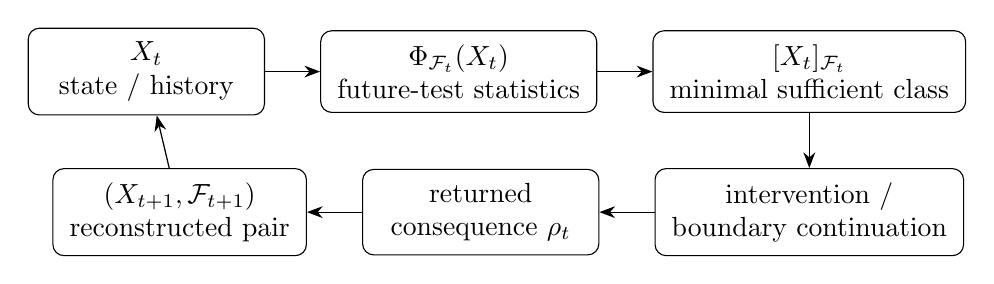
\begin{tikzpicture}[
  node distance=7mm and 7mm,
  box/.style={draw,rounded corners,align=center,inner xsep=6pt,inner ysep=5pt,minimum width=30mm},
  arr/.style={-{Stealth[length=2mm]},line width=0.45pt}
]
\node[box] (x) {$X_t$\\state / history};
\node[box,right=of x] (phi) {$\Phi_{\F_t}(X_t)$\\future-test statistics};
\node[box,right=of phi] (q) {$[X_t]_{\F_t}$\\minimal sufficient class};
\node[box,below=of q] (a) {intervention /\\boundary continuation};
\node[box,left=of a] (r) {returned\\consequence $\rho_t$};
\node[box,left=of r] (z) {$(X_{t+1},\F_{t+1})$\\reconstructed pair};
\draw[arr] (x) -- (phi);
\draw[arr] (phi) -- (q);
\draw[arr] (q) -- (a);
\draw[arr] (a) -- (r);
\draw[arr] (r) -- (z);
\draw[arr] (z) -- (x);
\end{tikzpicture}
\caption{The paper's core circulation. Compression is relative to an admitted family of future tests. Returned consequence may update the structural state, the test family, or both, so the next quotient need not preserve the previous partition.}
\label{fig:cycle}
\end{figure}

\section{Coupled dynamics of state and distinction}
\label{sec:dual-dynamics}

Most state-compression formalisms treat the relevance criterion as fixed. That is often appropriate for a stationary prediction task, but it hides a second dynamics. In an experiment, new apparatus can become available; in control, the objective or policy family can change; in a gauge theory, a different relational frame can expose a different algebra of observables; in quantum gravity, refinement can change the space of boundary continuations. The structural state and the distinction structure are then coupled.

Let
\begin{equation}
  Z_t=(X_t,\F_t).
\end{equation}
We write the most general discrete update schematically as
\begin{align}
 X_{t+1}
   &=\mathcal U(X_t,a_t,\rho_t;\F_t),
   \label{eq:structural-update}\\
 \F_{t+1}
   &=\mathcal G(\F_t,X_t,a_t,\rho_t;\mathcal C_t),
   \label{eq:test-update}
\end{align}
where $a_t$ is an intervention or continuation, $\rho_t$ a returned consequence, and $\mathcal C_t$ collects physical constraints on admissible testing such as available controls, boundary conditions, causal access, reference frame, resolution, and task. The semicolon is a reminder that $\F_t$ constrains which components of the structural update are operationally relevant, while the changed structure can alter which tests are physically available at the next stage.

This is not a second substance added to physics. $\F_t$ is a relational object: it encodes the family of distinctions that the current physical arrangement can make consequential. In an AI or control realization, $\mathcal C_t$ may include a task or policy family; in a physical realization it must be grounded in actual operations, boundary data, or relational observables. A purely verbal relabeling of $\F$ that changes no admissible statistics has no physical effect.

\begin{definition}[Relevance transition]
For a pair $x,y\in\Sspace$, a gauge-to-separator transition occurs at $t\to t+1$ when
\begin{equation}
  x\sim_{\F_t}y
  \quad\text{but}\quad
  x\not\sim_{\F_{t+1}}y.
  \label{eq:relevance-bifurcation}
\end{equation}
A separator-to-gauge transition is the reverse.
\end{definition}

The terminology is intentionally operational. A microscopic distinction has become newly consequential because the future family changed, not because the underlying past was rewritten. This distinction is useful whenever one wants to describe learning, experiment design, symmetry breaking, changing observational access, or boundary refinement without confusing changes of representation with changes of the represented system.

Two limiting cases recover familiar models. If $\F_{t+1}=\F_t$ for all $t$, only the structural state evolves and the quotient is fixed. If $X_{t+1}=X_t$ while $\F$ changes, the same physical state is being re-partitioned by a new question or access regime. The general case allows both to change.

\subsection{Quotient transport under evolving tests}

Let $U_t:\Sspace_t\to\Sspace_{t+1}$ be a physical or process evolution. Every test $T\in\F_{t+1}$ has a pullback through $U_t$ whenever the statistics of performing $T$ after $U_t$ can be represented as a test on the earlier state:
\begin{equation}
  P_{U_t^{\ast}T}(\cdot\mid x)
  :=
  P_T(\cdot\mid U_t x).
  \label{eq:test-pullback}
\end{equation}

\begin{proposition}[Quotient transport criterion]
\label{prop:quotient-transport}
The following are equivalent:
\begin{enumerate}[label=(\roman*)]
\item there exists a unique map $\overline U_t:\Q_{\F_t}\to\Q_{\F_{t+1}}$ satisfying
\begin{equation}
  \overline U_t\circ\pi_{\F_t}
  =
  \pi_{\F_{t+1}}\circ U_t;
  \label{eq:quotient-commute}
\end{equation}
\item $U_t$ preserves future-equivalence,
\begin{equation}
  x\sim_{\F_t}y
  \quad\Longrightarrow\quad
  U_t x\sim_{\F_{t+1}}U_t y;
  \label{eq:equiv-preservation}
\end{equation}
\item for every $T\in\F_{t+1}$, the later outcome law after $U_t$ is constant on the earlier quotient classes, i.e. there exists a map $g_T$ on $\Q_{\F_t}$ such that
\begin{equation}
  P_T(\cdot\mid U_t x)=g_T([x]_{\F_t})
  \qquad\forall x\in\Sspace_t.
  \label{eq:test-factorization}
\end{equation}
\end{enumerate}
A sufficient condition for these equivalent statements is the literal pullback closure
\begin{equation}
  U_t^{\ast}\F_{t+1}\subseteq\F_t.
  \label{eq:pullback-closure}
\end{equation}
\end{proposition}

\begin{proof}
Statements (i) and (ii) are the standard descent condition for a map on equivalence classes: (i) implies (ii) because equal earlier classes have equal images under $\overline U_t$, while (ii) makes $\overline U_t([x]_{\F_t}):=[U_t x]_{\F_{t+1}}$ well defined and unique. Statements (ii) and (iii) are equivalent by the definition of $\sim_{\F_{t+1}}$: every later test statistic must take the same value on every earlier equivalence class. Finally, if \eqref{eq:pullback-closure} holds and $x\sim_{\F_t}y$, then for each $T\in\F_{t+1}$,
\[
P_T(\cdot\mid U_t x)
=P_{U_t^{\ast}T}(\cdot\mid x)
=P_{U_t^{\ast}T}(\cdot\mid y)
=P_T(\cdot\mid U_t y),
\]
so (ii) follows.
\end{proof}

The abstract descent condition is not claimed as a new theorem of quotient theory. Classical Markov-chain lumpability is a close special case: a partition supports closed reduced dynamics only when states inside one lump induce the same transition probabilities over future lumps~\cite{jernigan2003}. The present formulation changes the emphasis by indexing equivalence to an explicit operational test family that may itself evolve.

The converse obstruction is equally useful. If $x\sim_{\F_t}y$ but some $T\in\F_{t+1}$ distinguishes $U_t x$ from $U_t y$, then no map on the old quotient classes can reproduce the new predictions. The later test has reopened a distinction that the earlier quotient erased. The remedy is not interpretive: refine the earlier state representation, enlarge the earlier test family when physically justified, or accept that the old quotient was task-local rather than dynamically sufficient.

\begin{example}[Quantum channels: states forward, effects backward]
Let $U_t=\mathcal E_t$ be a completely positive trace-preserving map. A later effect $E$ pulls back by the Heisenberg adjoint,
\begin{equation}
  E\longmapsto \mathcal E_t^{\dagger}(E),
  \qquad
  \Tr[E\,\mathcal E_t(\rho)]
  =
  \Tr[\mathcal E_t^{\dagger}(E)\rho].
  \label{eq:heisenberg-pullback}
\end{equation}
Therefore Proposition~\ref{prop:quotient-transport} applies whenever
\begin{equation}
  \mathcal E_t^{\dagger}(\F_{t+1})\subseteq\F_t.
  \label{eq:quantum-pullback-closure}
\end{equation}
For a qubit dephasing channel in the $Z$ basis and a future family containing only $Z$-diagonal effects, the pullback remains $Z$-diagonal and phase coherence may be safely absent from the operational quotient. By contrast, under identity evolution with $\F_t$ containing only $Z$ tests and $\F_{t+1}$ enlarged to include an $X$ test, the states $|+\rangle$ and $|-\rangle$ are equivalent at $t$ but distinguishable at $t+1$. Equation \eqref{eq:pullback-closure} fails exactly because the new $X$ effect was not represented by the earlier test family.
\end{example}

The adjoint relation in \eqref{eq:heisenberg-pullback} is standard Schrödinger--Heisenberg duality. Its role here is not to rename that duality, but to expose exactly when a changing family of operational distinctions is compatible with quotienting the simultaneously evolving state.

This forward-state/backward-test relation is the precise sense in which structural dynamics and distinction dynamics are coupled. The physical state propagates forward; later operational questions pull backward through the dynamics. A quotient is dynamically legitimate only when these two directions commute.

\subsection{A consistency condition}

The pair dynamics becomes self-sealing if $\mathcal G$ is permitted to delete every test that contradicts the current compressed state. A minimal nontriviality condition is therefore to retain independently available separators. Let $\F^{\mathrm{ext}}_{t+1}$ denote tests made available by the physical environment, another subsystem, a held-out experiment, or an externally specified task. Then a corrigible update should satisfy
\begin{equation}
  T\in\F^{\mathrm{ext}}_{t+1}
  \;\land\;
  D_T\!\left(P_T(\cdot\mid X_t),P_T(\cdot\mid X_t\oplus\rho_t)\right)>\eps
  \quad\Longrightarrow\quad
  T\notin\mathcal G_{\mathrm{erase}}
  \label{eq:no-self-seal}
\end{equation}
for the declared tolerance $\eps$, unless a separately justified physical constraint makes the test inadmissible. In plainer terms, the model may change what it asks, but it may not manufacture agreement by deleting a still-available discriminator.

\section{Relational observables and indexed physical description}
\label{sec:relational}

General covariance makes the index of a description physical rather than merely psychological. Coordinates in general relativity are gauge labels; observables must be constructed relationally or through gauge-invariant combinations. Rovelli's partial-observable program and Dittrich's complete observables provide influential formulations of this problem~\cite{rovelli2002,dittrich2006}. Quantum reference-frame work makes the reference system itself part of the quantum description and studies transformations between different frame-relative state assignments~\cite{giacomini2019,vanrietvelde2020}. Particularly close to the present quotient, G\l{}owacki constructs operational quantum frames by quotienting state spaces under indistinguishability by available relative effects, and Carette, G\l{}owacki, and Loveridge develop frame transformations directly between equivalence classes of such relative states~\cite{glowacki2023,carette2025}. Recent work by Thiemann develops operational reference frames, relational observables, gauge reduction, and transformations between relational frames in a general field-theoretic setting that includes general relativity coupled to matter~\cite{thiemann2026}.

Let $i$ denote a physically specified relational reference system. The future map becomes
\begin{equation}
  \Phi_{\F,i}(X)
  :=
  \bigl(P_T(\cdot\mid X,i)\bigr)_{T\in\F_i}.
  \label{eq:indexed-future}
\end{equation}
There is no requirement that
\begin{equation}
  [X]_{\F_i,i}=[X]_{\F_j,j}.
\end{equation}
What is required is a lawful transformation between descriptions when the theory supplies a change of relational frame. The quotient should therefore be covariant in the operational sense: frame changes may alter representatives, accessible observables, and even the apparent partition, while preserving shared observable predictions after translating the tests themselves.

This matters for the interpretation of ``observer-relative compression.'' The observer in the present formalism is not assumed to be conscious, human, or epistemically privileged. It is an indexed physical interface or reference system. The same formal slot can be occupied by a laboratory, clock field, material reference system, boundary component, or controlled subsystem. Any stronger interpretation requires additional evidence.

\section{Relational nonfactorization and carrier-substitution tests}
\label{sec:nonfactor}

Coupling alone does not imply that a joint system requires a genuinely relational state coordinate. Two components can interact strongly while all admitted joint predictions remain reconstructible from sufficient local states plus a known composition rule. A stronger question is whether the complete local operational descriptions are themselves sufficient for the declared joint future.

Let $\Sspace_{AB}$ be a joint state or history space with local projection maps
\begin{equation}
  m_A:\Sspace_{AB}\to\Sspace_A,
  \qquad
  m_B:\Sspace_{AB}\to\Sspace_B.
  \label{eq:local-projections}
\end{equation}
Let $\F_A$ and $\F_B$ be local future-test families and let $\F_{AB}$ be a family of admitted joint tests. Define the product of local future-sufficient descriptions by
\begin{equation}
  R_{\mathrm{loc}}(x)
  :=
  \bigl(
    [m_A(x)]_{\F_A},
    [m_B(x)]_{\F_B}
  \bigr).
  \label{eq:local-quotient-pair}
\end{equation}
The joint future map is $\Phi_{\F_{AB}}: \Sspace_{AB}\to\Y_{\F_{AB}}$.

\begin{definition}[Operational relational factorization]
The declared joint description is \emph{relationally reducible} when there exists a map $g$ such that
\begin{equation}
  \Phi_{\F_{AB}}
  =
  g\circ R_{\mathrm{loc}}.
  \label{eq:relational-factorization}
\end{equation}
It is \emph{operationally relationally nonfactorizable} relative to $(\F_A,\F_B,\F_{AB})$ when no such $g$ exists.
\end{definition}

\begin{proposition}[Separating witness for relational nonfactorization]
\label{prop:relational-witness}
Operational relational nonfactorization holds if and only if there exist $x,y\in\Sspace_{AB}$ such that
\begin{equation}
  R_{\mathrm{loc}}(x)=R_{\mathrm{loc}}(y)
  \quad\text{but}\quad
  \Phi_{\F_{AB}}(x)\neq\Phi_{\F_{AB}}(y).
  \label{eq:relational-witness}
\end{equation}
\end{proposition}

\begin{proof}
A factorization through $R_{\mathrm{loc}}$ exists exactly when $\Phi_{\F_{AB}}$ is constant on every fiber of $R_{\mathrm{loc}}$. Equation~\eqref{eq:relational-witness} is precisely a witness that this constancy fails.
\end{proof}

The criterion is deliberately operational. It does not say that the two local components have fused, that one global agent exists, or that the microscopic carrier is ordinary quantum mechanics. Classical common causes, shared memory, latent environmental variables, and explicit interaction histories can all make joint futures depend on information absent from separately chosen local state descriptions. Conversely, a Hilbert-space quantum state can be entangled while a restricted operational family fails to reveal that entanglement. The present factorization criterion is therefore broader than physical quantum separability, but it overlaps the established notion of generalized entanglement when a composite system has local observables that fail to determine a globally constrained state~\cite{filkromer2011}. The carrier must decide which notion is physically warranted.

For the approximate case, define a relational-separation radius
\begin{equation}
  \Delta_{\mathrm{rel}}
  :=
  \sup\left\{
  d_{\F_{AB}}(x,y):
  d_{\F_A}(m_Ax,m_Ay)=0,
  \ d_{\F_B}(m_Bx,m_By)=0
  \right\}.
  \label{eq:relational-radius}
\end{equation}
Whenever the relevant distances are finite, $\Delta_{\mathrm{rel}}>0$ exhibits joint operational structure invisible to both local quotient states. The quantity is indexed to the chosen test families; changing the admissible joint tests can create or remove the separation.

\subsection{Causal enrichment and nested shared-world null models}
\label{sec:causal-enrichment}

Failure of Equation~\eqref{eq:relational-factorization} is only as informative as the local state descriptions supplied to it. If a shared cause, interaction history, communication channel, environmental trace, or network-mediated dependency is omitted from the state, the missing variable can masquerade as an irreducible relation. This is especially important for biological and social systems, which are embedded in common environments and persistent communication networks rather than sampled as isolated pairs.

Let
\begin{equation}
  H:\Sspace_{AB}\to\mathcal H
  \label{eq:shared-history-map}
\end{equation}
collect a declared shared-history / common-cause state. Depending on the carrier, $H$ may contain prior interaction, common stimuli, communication records, environmental variables, shared memory, technical-network traces, or other independently motivated causal coordinates. Define the enriched representation
\begin{equation}
  R_{\mathrm{enr}}(x)
  :=
  \bigl(
    [m_A(x)]_{\F_A},
    [m_B(x)]_{\F_B},
    H(x)
  \bigr).
  \label{eq:enriched-representation}
\end{equation}
We say that a joint future map is \emph{residually nonfactorizable after enrichment} when no map $g_{\mathrm{enr}}$ satisfies
\begin{equation}
  \Phi_{\F_{AB}}
  =
  g_{\mathrm{enr}}\circ R_{\mathrm{enr}}.
  \label{eq:enriched-nonfactorization}
\end{equation}
Equivalently, there must exist $x,y$ with $R_{\mathrm{enr}}(x)=R_{\mathrm{enr}}(y)$ but $\Phi_{\F_{AB}}(x)\neq\Phi_{\F_{AB}}(y)$.

The resulting claim strength is monotone under nested enrichment. If $H_2=(H_1,K)$ contains every coordinate in $H_1$ plus additional independently justified information, then factorization through the coarser representation built from $H_1$ implies factorization through the finer representation built from $H_2$. Therefore,
\begin{equation}
  \text{nonfactorization after }H_2
  \Longrightarrow
  \text{nonfactorization after }H_1.
  \label{eq:enrichment-monotonicity}
\end{equation}
Survival under a richer null model is thus a strictly stronger evidential statement. In applications one should report the enrichment level at which factorization first succeeds or, if it does not, which shared variables have actually been ruled out. The framework does not license an ``unknown cause therefore nonlocal'' inference.

This enrichment step also makes multiscale embedding explicit. A dyad can be simultaneously embedded in a laboratory, family, social network, technological platform, ecological niche, or other shared carrier. Those larger structures belong in $H$ whenever they can alter the joint future statistics. Only the residual left after such channels are represented is eligible for a stronger generalized-nonseparability interpretation.

\subsection{Generalized entanglement and synchronistic event witnesses}
\label{sec:synchronicity}

The relation between nonseparability and synchronicity has a substantial prior literature and should not be introduced as a new analogy. The Pauli--Jung program treated mental and material descriptions as complementary aspects of an underlying psychophysically neutral order, and later work developed structural typologies of mind--matter correlations in that dual-aspect setting~\cite{atmanspacherfach2013,atmanspacher2014}. In GQT, a composite system admits identifiable subsystems with mutually compatible local observables, together with a global observable of the whole that is complementary to those local observables. A generalized entangled state is then an eigenstate of the global observable without being an eigenstate of the corresponding local observables~\cite{atmanspacher2002,filkromer2011}. The formalism was designed precisely to retain a well-defined notion of complementarity and entanglement after dropping structures special to microscopic quantum physics. Von Lucadou, Römer, and Walach subsequently interpreted synchronistic phenomena as entanglement correlations in this generalized sense and imposed a no-transmission condition forbidding their use as controllable signals~\cite{lucadou2007}. This is established prior art for the structural claim, not evidence that reported human synchronicities are Hilbert-space quantum entanglement.

The present quotient language recovers the core nonseparability statement in a test-relative form. If the local families $\F_A$ and $\F_B$ exhaust the declared local observables, while a global test $T_G\in\F_{AB}$ distinguishes joint states that have the same local quotient pair, then $T_G$ is a witness of Equation~\eqref{eq:relational-witness}. In other words, the local operational states fail to determine the joint operational state. GQT reaches a related conclusion from global/local complementarity; the present criterion does not require noncommuting observables and is therefore formally broader.

A realized event should be called a \emph{synchronistic relational witness} here only when two independent requirements are kept separate. First, it must instantiate relational separation: the relevant joint test distinguishes histories that are identical under the declared local quotient pair. For a stronger claim, the same separation must survive the causal-enrichment test of \Cref{sec:causal-enrichment}, so that explicitly modeled shared history, communication, environmental structure, and network traces do not already restore factorization. Second, its returned consequence must remain future-separating,
\begin{equation}
  \rho\in\Res_{\F_{AB}}(C),
  \label{eq:synch-residual}
\end{equation}
so that the event changes an admitted continuation, reachability relation, prediction, or lawful response rather than merely attracting retrospective attention. An \emph{entanglement-like} interpretation adds the further no-transmission obligation that admissible manipulations of either subsystem cannot be used to control the marginal outcome law of the other. None of these conditions alone establishes Bell nonlocality or an ordinary quantum carrier.

This formulation also exposes the strongest ordinary rival. Empirical psychology operationalizes synchronicity as a conjunction of event awareness and subsequent meaning-detection rather than as a demonstrated nonlocal mechanism~\cite{russonetzer2023}. A 2026 matched study of ultra-Orthodox and secular participants found similar levels of synchronicity awareness and meaning-detection across the groups, while the relation between attachment to God and meaning in life depended on meaning-detection rather than awareness alone~\cite{russonetzer2026}. This supports a useful separation between occurrence, interpretation, and downstream consequence; it does not test relational nonfactorization. More strongly, a recent biosemiotic account explains synchronistic experience through anticipation, salience alignment, memory, communication, niche construction, and causal opacity without requiring acausal order~\cite{mccoss2026}. Under the present framework such mechanisms belong inside $H$ before nonfactorization is assessed. A subjective synchronistic experience is therefore not itself evidence for Equation~\eqref{eq:relational-witness}; the stronger claim survives only if an adequately enriched causal state still fails the factorization test.

\subsection{Carrier substitution as a discriminator}

A shared diagrammatic shape is not sufficient to identify mechanisms across domains. We will call a proposed carrier substitution \emph{structure-preserving} only when an explicit bridge preserves, to the claimed accuracy, at least
\begin{equation}
\begin{aligned}
&\text{indexed local components and their projection maps},\\
&\text{the admitted local and joint tests and their outcome laws},\\
&\text{the local and joint quotient relations},\\
&\text{composition or quotient transport under the relevant dynamics},\\
&\text{and the separating witnesses that would falsify the identification}.
\end{aligned}
\label{eq:carrier-substitution}
\end{equation}
A correspondence that preserves only visual geometry, terminology, or an endpoint state is therefore insufficient. The point of the criterion is to distinguish a reusable invariant from an attractive analogy.

Recent neuroscience provides useful partial stress tests because it exhibits distributed, history-bearing spatiotemporal organization without thereby supplying a quantum or gravitational mechanism. Spiral-like cortical waves propagate around phase-singularity centres, interact across scales, and show task-dependent organization~\cite{xu2023}. A recent review emphasizes that cortical traveling waves introduce spatiotemporal dependencies not naturally captured by purely feedforward or feedback descriptions and can embed sensory history in evolving activity patterns~\cite{muller2026}. Human intracranial recordings further show that co-occurring ripple oscillations coordinate long-range, stimulus-specific neuronal co-firing during working memory~\cite{verzhbinsky2026}, while sustained visual perception exhibits stable distributed content representations in occipitotemporal regions and more transient onset-related representations in frontoparietal regions~\cite{vishne2023}. At the interpersonal scale, hyperscanning research studies neural and behavioral processes that extend across interacting partners, with cross-brain synchrony implicated in communication, coordination, and learning~\cite{schilbach2025}. At a still larger scale, social-network topology changes how memories, beliefs, and problem-solving information are integrated across human groups~\cite{momennejad2022}. These results instantiate some slots in Equation~\eqref{eq:carrier-substitution}, including distributed local activity, temporal organization, coordination, retained interaction history, and multiscale embedding. They also illustrate why the enrichment state $H$ cannot be omitted when testing human dyads: shared stimuli, reciprocal behavior, social topology, and technological communication can all generate joint dependence. None of these results by themselves establish Equation~\eqref{eq:relational-witness}, quantum process nonseparability, or a theory of consciousness. In particular, a spiral phase singularity is an organizing locus of a wave field, not automatically a fixed point in the dynamical-systems sense.

A recent and independent quantum-foundations proposal gives a different comparator. Pettini considers a warped $(3,2)$-dimensional spacetime in which local four-dimensional detector readouts are projections of a shared bulk field; the model explicitly distinguishes a factorized sector from a proposed non-separable contextual drive and predicts a distance-dependent cross-pair correlation absent for independently prepared Bell pairs in standard quantum mechanics~\cite{pettini2026}. This supplies a concrete example of the logical pattern ``distinct local projections plus a nonfactorizing higher-dimensional carrier.'' It is not evidence for the present quantum-gravity proposal, for a preferred ontology of observers, or for any neural realization. Its relevance here is narrower: it shows how the factorization discriminator can be attached to a carrier-specific dynamical hypothesis with an independent experimental failure condition.

\section{Boundary quantum gravity and future-sufficient coarse graining}
\label{sec:qg}

Spin-foam models provide a covariant path-integral formulation related to loop quantum gravity. Their amplitudes are associated with combinatorial two-complexes and boundary spin-network data; in geometric sectors, intertwiners admit an interpretation in terms of quantum polyhedra~\cite{perez2013,eprl2008,freidelkrasnov2008,bianchi2011}. Entanglement can encode gluing relations among neighboring quantum polyhedra~\cite{baytas2018}. Independently, boundary modes in gravity have been shown to act as quantum reference frames for local gravitational symmetries~\cite{kabel2023}. These results make boundary composition and relational access central rather than incidental.

The continuum problem is correspondingly a problem of refinement. A discretization $\Delta$ supplies a boundary state space $\Sspace_{\Delta}$ and an amplitude or process assignment. Refinement $\Delta\preceq\Delta'$ adds microscopic boundary or bulk structure. Let
\begin{equation}
  C_{\Delta'\to\Delta}:\Sspace_{\Delta'}\to\overline{\Sspace}_{\Delta}
  \label{eq:qg-coarse-map}
\end{equation}
be a candidate fine-to-coarse map into a coarse state space $\overline{\Sspace}_{\Delta}$; the model may later identify this space with a preferred kinematical or physical state space. Background-independent renormalization programs formulate related consistency problems through boundary data, embedding maps, and cylindrical consistency~\cite{dittrich2012,dittrichsteinhaus2014,steinhaus2020}.

Let $\F_{\Delta}$ be a physically justified family of future boundary continuations and measurements available at the coarse boundary. Assume both the fine and coarse descriptions assign outcome laws to each $T\in\F_{\Delta}$:
\begin{align}
  \Phi_{\F_{\Delta}}^{\Delta'}(x)
  &=\bigl(P_{T}^{\Delta'}(\cdot\mid x)\bigr)_{T\in\F_{\Delta}},\\
  \overline\Phi_{\F_{\Delta}}^{\Delta}(u)
  &=\bigl(\overline P_{T}^{\Delta}(\cdot\mid u)\bigr)_{T\in\F_{\Delta}}.
  \label{eq:qg-future-maps}
\end{align}

\begin{conjecture}[Future-sufficient coarse-graining principle]
\label{conj:fscp}
For each admissible refinement $\Delta\preceq\Delta'$ and physically justified family $\F_{\Delta}$, an exact minimal coarse-graining map $C^{\F}_{\Delta'\to\Delta}$, when it exists, should satisfy two independent requirements:
\begin{align}
\text{prediction preservation: }&
\Phi_{\F_{\Delta}}^{\Delta'}
=
\overline\Phi_{\F_{\Delta}}^{\Delta}
\circ C^{\F}_{\Delta'\to\Delta},
\label{eq:fscp-sufficiency}\\
\text{minimality: }&
C^{\F}_{\Delta'\to\Delta}(x)
=C^{\F}_{\Delta'\to\Delta}(y)
\Longleftrightarrow
x\sim_{\F_{\Delta}}y.
\label{eq:fscp-minimality}
\end{align}
Thus the coarse state is sufficient for every admitted future continuation and carries no additional independent coordinate that separates states invisible to all such continuations, unless another explicitly stated physical constraint requires it.
\end{conjecture}

The two clauses must not be collapsed. Equation \eqref{eq:fscp-sufficiency} can hold for a representation that retains redundant microscopic information; equation \eqref{eq:fscp-minimality} can hold for a quotient that has not yet been equipped with a physically correct coarse prediction map. Together they identify the coarse state space with the operational quotient up to a change of coordinates.

For approximate calculations, define the prediction error of a coarse map by
\begin{equation}
  \operatorname{Err}_{\F_{\Delta}}(C)
  :=
  \sup_{x\in\Sspace_{\Delta'}}
  \sup_{T\in\F_{\Delta}}
  D_T\!\left(
    P_T^{\Delta'}(\cdot\mid x),
    \overline P_T^{\Delta}(\cdot\mid Cx)
  \right).
  \label{eq:qg-approx-error}
\end{equation}
An $\eps$-sufficient map has $\operatorname{Err}_{\F_{\Delta}}(C)\le\eps$; approximate minimality is then a separate rate--distortion or model-selection problem rather than something smuggled into the same inequality.

A viable refinement family must also obey structural obligations. First, equivalence must survive admitted composition: if $R$ is a common boundary continuation that maps states on $\Delta$ to a later boundary $\Delta_R$, then
\begin{equation}
  x\sim_{\F_{\Delta}}y
  \quad\Longrightarrow\quad
  R\circ x\sim_{\F_{\Delta_R}}R\circ y
  \label{eq:qg-composition-closure}
\end{equation}
for every continuation that the claimed coarse theory treats as admissible. This is the boundary version of Proposition~\ref{prop:quotient-transport}.

Second, whenever the fine-to-coarse maps descend to quotient maps $\overline C_{\Delta'\to\Delta}$, successive refinements should form a coherent projective diagram:
\begin{equation}
  \overline C_{\Delta''\to\Delta}
  =
  \overline C_{\Delta'\to\Delta}
  \circ
  \overline C_{\Delta''\to\Delta'}
  \qquad
  (\Delta\preceq\Delta'\preceq\Delta'').
  \label{eq:qg-projective}
\end{equation}
Third, a lawful change of physical reference frame should itself satisfy the quotient-transport criterion after translating the corresponding test family. Finally, any candidate continuum object must recover the appropriate relational observables, correlations, and dynamics of general relativity in its semiclassical regime.

The variance of the continuum construction should not be guessed from notation. Fine-to-coarse maps such as \eqref{eq:qg-coarse-map} naturally define a projective system; coarse-to-fine embedding maps used elsewhere in loop quantum gravity naturally support inductive constructions. The relevant category, maps, topology, and convergence notion must therefore be supplied by the chosen quantum-gravity model before one writes a specific limit.

\subsection{Why the 2026 continuum result matters}

Bruno \emph{et al.} formulate spin-foam continuum limits axiomatically using Hilbert spaces and amplitudes associated with triangulated boundary data. Under natural strong convergence assumptions they prove a no-go result: sufficiently strong convergence drives the continuum theory to a topological one. They therefore examine weaker distributional convergence, with the cylinder amplitude acting as a rigging map onto a physical Hilbert space~\cite{bruno2026}. The result does not imply that future-sufficient quotients solve the obstruction. It identifies exactly the kind of mistake a coarse-graining criterion must avoid: imposing a notion of convergence so strong that physically consequential local structure is silently erased.

The proposed criterion attacks a different question. Instead of asking whether all microscopic data converge strongly, ask which distinctions survive all physically admissible future continuations. If a degree of freedom is future-invisible, retaining it is unnecessary for the declared operational theory. If it changes a future boundary statistic, a coarse graining that deletes it has lost physical content. This criterion can be compared directly with cylindrical consistency and with the physical Hilbert space produced by distributional limits.

\subsection{Polyhedra are a donor, not a proof}

The polyhedral interpretation of intertwiners is structurally suggestive because local faces, boundary data, gluing, and coarse composition already have precise meanings in loop quantum gravity~\cite{bianchi2011,baytas2018}. But geometrical resemblance is not evidence that an independently developed polyhedral state model is physically realized by LQG. A bridge earns physical status only if it preserves states, observables, composition, boundary data, dynamics, and semiclassical behavior. Removing interpretive labels while leaving the mathematics and predictions unchanged is therefore a useful negative control.

\section{AI and control: mature realizations of the same quotient pattern}
\label{sec:ai}

The AI literature is useful here because it has already confronted the practical version of the same question: what is the smallest state representation that remains sufficient for future behavior?

Computational mechanics defines causal states by an equivalence relation on histories: two pasts belong to the same causal state when they induce the same conditional distribution over futures. The resulting $\epsilon$-machine is minimal among equally predictive representations under the theory's assumptions~\cite{crutchfield1989,shalizi2001}. Predictive-state representations replace hidden latent states with predictions of outcomes of future experiments and can represent controlled dynamical systems directly through observable tests~\cite{littman2001,singh2004}. These are exceptionally close mathematical neighbors of \eqref{eq:future-equivalence}.

Markov decision-process abstraction adds action and value relevance. Givan, Dean, and Greig develop equivalence relations and minimization procedures in which aggregated states preserve the properties needed to induce optimal policies~\cite{givan2003}. Bisimulation metrics extend this idea quantitatively and give bounds connecting state similarity to value functions~\cite{ferns2011}. Information-bottleneck work asks which information about a past should be retained because it predicts the future, explicitly trading complexity against predictive power~\cite{tishby1999,creutzig2009}. Still \emph{et al.} connect nonpredictive stored information to thermodynamic inefficiency in driven systems~\cite{still2012}.

These antecedents mean that a future-sufficient quotient should not be advertised as a new invention of predictive state abstraction. Its cross-domain role is instead diagnostic. It exposes which part of a proposed physics construction is ordinary sufficient-state mathematics and which part is genuinely new physical structure.

\subsection{Learned representations with an evolving test family}

The transport theorem of \Cref{sec:dual-dynamics} also suggests an algorithmic object: learned representations should be revised whenever newly admissible tests fail to pull back to distinctions represented by the current state abstraction. Let $h_t$ be an observed history and $z_t=f_{\theta}(h_t)$ a learned representation. For a current test distribution $T\sim\F_{\eta,t}$, train a predictor $p_{\theta}(o\mid z,T)$ by minimizing
\begin{equation}
  \mathcal L_{\mathrm{pred}}(\theta;\eta)
  =
  \mathbb E_{h,T}
  D\!\left(
    P_T(\cdot\mid h),
    P_{\theta}(\cdot\mid f_{\theta}(h),T)
  \right).
  \label{eq:pred-loss}
\end{equation}
Compression can be added through a complexity penalty $\Omega(f_{\theta})$ or information bottleneck. The complementary update searches for tests that expose distinctions the current representation has incorrectly collapsed:
\begin{equation}
  \eta_{t+1}
  \in
  \arg\max_{\eta\in\mathcal A_t}
  \mathbb E_{h,h'}
  \left[
  \mathbf 1\{f_{\theta}(h)=f_{\theta}(h')\}
  d_{\F_{\eta}}(h,h')
  \right],
  \label{eq:test-search}
\end{equation}
subject to an admissibility set $\mathcal A_t$ that prevents the test generator from inventing impossible interventions or reading evaluator-only information.

Equations \eqref{eq:pred-loss}--\eqref{eq:test-search} implement a bounded alternation:
\begin{equation}
  \text{compress for current tests}
  \longleftrightarrow
  \text{search for admissible separating tests}.
  \label{eq:alternation}
\end{equation}
The representation becomes more independent of a fixed teacher-supplied vocabulary because new discriminators can be generated from held-out consequences rather than from answer-shaped labels. But the external environment remains indispensable: a learner may generate a test or method, yet it does not author the returned evidence that the method works.

\begin{table}[t]
\caption{Carrier-substituted realizations of the same future-equivalence pattern. The table asserts a shared mathematical form, not mechanism identity.}
\label{tab:cross-domain}
\centering
\small
\begin{tabular}{@{}p{0.18\linewidth}p{0.22\linewidth}p{0.24\linewidth}p{0.24\linewidth}@{}}
\toprule
Domain & State/history object & Future tests & Quotient meaning \\
\midrule
Computational mechanics & observed past & conditional future events & causal state \\
Predictive-state control & action-observation history & executable tests / action sequences & predictive state \\
MDP abstraction & environment state & policies, rewards, transitions & behavioral equivalence / bisimulation class \\
Quantum process theory & process tensor / comb & multitime instruments & operational process class \\
Boundary quantum gravity & boundary state / amplitude data & admissible future continuations & proposed future-sufficient coarse state \\
\bottomrule
\end{tabular}
\end{table}

\section{Falsifiers, reductions, and non-entailments}
\label{sec:falsifiers}

A useful synthesis should make itself easier to remove. The following outcomes would weaken, reduce, or falsify the quantum-gravity proposal.

First, the future-test quotient may add no structure beyond an existing mature construction. If a standard cylindrical-consistency or renormalization map can be shown to satisfy the same universal property with the same physically justified tests, the new terminology should be retired and the result stated in the mature language.

Second, the physically admissible test family may be impossible to define without presupposing the continuum theory it is meant to construct. This would make the criterion circular. A viable implementation needs finite/refined boundary tests whose translation across discretizations is defined independently enough to evaluate coarse graining.

Third, quotient preservation may conflict with composition. If two boundary states are indistinguishable under all local admitted tests but become distinguishable after gluing to a common region, then the original test family was not compositionally closed. The cure is not to declare the distinction gauge; it is to enlarge $\F$ or abandon the coarse identification.

Fourth, a candidate continuum quotient may fail the semiclassical limit. Preserving a set of quantum tests is insufficient if the resulting large-scale state space does not reproduce the appropriate relational observables, correlations, and dynamics of general relativity.

Fifth, the coupled $\F_t$ dynamics may be unnecessary in a target domain. If every physically relevant discriminator can be fixed once and for all, then \eqref{eq:test-update} is surplus structure and should be frozen. Conversely, if $\F_t$ is allowed to change arbitrarily, the theory becomes vacuous because any failed prediction can be hidden by redefining what matters. Equation \eqref{eq:no-self-seal} exists precisely to block that move.

Several stronger claims do not follow from the framework:
\begin{equation}
\begin{aligned}
\text{operational quotient} &\not\Rightarrow \text{quantum measurement collapse},\\
\text{indexed reference frame} &\not\Rightarrow \text{conscious observer},\\
\text{shared quotient structure} &\not\Rightarrow \text{shared physical mechanism},\\
\text{relational nonfactorization} &\not\Rightarrow \text{Hilbert-space quantum entanglement},\\
\text{experienced synchronicity} &\not\Rightarrow \text{relational nonfactorization},\\
\text{generalized entanglement} &\not\Rightarrow \text{Bell nonlocality},\\
\text{cross-carrier recurrence} &\not\Rightarrow \text{mechanism identity},\\
\text{spin-foam compatibility} &\not\Rightarrow \text{continuum existence},\\
\text{future-sufficient compression} &\not\Rightarrow \text{unique test family}.
\end{aligned}
\label{eq:nonentailments}
\end{equation}
These fences are part of the theory rather than apologies around it. They specify which experiments or proofs are still required.

\section{Discussion}

Four observations survive the comparison across fields. The first is mathematical: a declared family of future tests induces a canonical equivalence relation, and its quotient is the coarsest exact representation sufficient for those tests. This is not a speculative principle. It is a direct factorization result with mature relatives in statistics, dynamical systems, AI, and operational physics.

The second observation is dynamical and exact. A state representation and the family of distinctions by which it is judged need not evolve on separate conceptual floors. The quotient-transport theorem identifies the compatibility condition: later tests must pull back through the structural dynamics to distinctions represented by the earlier test family. Physical states propagate forward while tests pull backward. When this condition fails, quotient evolution is not well defined because a later admissible experiment can reopen a distinction that an earlier compression erased. The pair $(X_t,\F_t)$ is therefore more than notation for two changing lists; it carries a commuting condition between structural evolution and operational distinction.

The third observation concerns relational organization. A coupled pair need not define a new irreducible operational state, but when the joint future map fails to factor through the product of the local future-sufficient quotients, the relation carries consequential information that the two local descriptions do not contain separately. This criterion is distinct from Hilbert-space entanglement but intersects the older GQT notion of generalized entanglement, where a globally constrained state is not determined by local subsystem states~\cite{filkromer2011}. The synchronicity literature makes that overlap historically important rather than terminological: synchronistic phenomena have already been modeled as generalized entanglement correlations~\cite{lucadou2007}. The present contribution is to add explicit future-test quotients, evolving test families, multitime transport, a returned-consequence discriminator, and a nested causal-enrichment test. A reported meaningful coincidence enters the stronger class only after ordinary shared-history, common-cause, communication, environmental, and salience mechanisms are represented and the remaining joint prediction still fails factorization. This turns the shared-world objection from a verbal caveat into part of the formal null model.

The fourth observation concerns quantum gravity. Coarse graining on a background-independent boundary theory needs a criterion for which distinctions are expendable. ``Microscopic'' is not enough, because a fine degree of freedom can remain observable after composition. ``Gauge'' is not enough unless the gauge relation has already been physically established. Future-equivalence supplies a test: erase a distinction only when all admitted future continuations agree that it makes no difference. This is compatible in spirit with the boundary-centered renormalization literature, but it sharpens the retention rule into an operational quotient.

The difficult work remains. A spin-foam implementation must specify the admissible tests, their translation between refinements, the probability interpretation, and their closure under composition. It must compare the resulting quotient with existing embedding-map and rigging-map constructions, then recover a suitable semiclassical gravitational regime. The 2026 continuum no-go result makes these requirements more, not less, important: an over-strong convergence rule can erase too much structure, while an under-constrained one may preserve discretization artifacts~\cite{bruno2026}.

There is also a methodological consequence. Cross-domain recurrence should be tested by carrier substitution rather than protected by terminology. Remove the words ``predictive state,'' ``quantum process,'' or ``future-sufficient.'' If the same equivalence, composition law, discriminator, and failure condition can be reconstructed in a new carrier, the shared mathematical structure survives. If the labels are doing the work, the bridge has failed.

\section{Conclusion}

The central construction of this paper is deliberately small:
\begin{equation}
  x\sim_{\F}y
  \quad\Longleftrightarrow\quad
  \text{every admitted future test assigns }x\text{ and }y\text{ the same consequences}.
\end{equation}
Its quotient is the minimal exact $\F$-sufficient state. Its pseudometric extension measures approximate distinguishability. The quotient-transport theorem adds the dynamical condition: an evolution descends to quotient states when every later admitted test is constant on earlier quotient classes; literal pullback closure is a sufficient operational realization. Quantum channels express this through the dual action of a channel on states and its Heisenberg adjoint on effects. For joint systems, the additional factorization discriminator asks whether all admitted joint futures can be reconstructed from the product of the local future-sufficient states. The causal-enrichment ladder then asks whether any apparent failure survives progressively richer shared-history and common-cause descriptions. Residual failure identifies relational operational structure without, by itself, selecting a microscopic mechanism. In the special case where a future-separating returned event also witnesses this enriched failure, the framework supplies an event-level notion of a synchronistic relational witness. Existing GQT work already interprets synchronicity through generalized entanglement; the present formulation adds the temporal and operational conditions needed to distinguish a consequential nonfactorizing return from ordinary coincidence, salience, shared causal history, or network-mediated dependence.

The quantum-gravity claim is deliberately narrower: spin-foam coarse graining should preserve admitted boundary-test statistics and should erase exactly the distinctions those tests cannot separate, while remaining stable under composition and refinement and recovering the appropriate semiclassical gravitational observables. Whether a nontrivial spin-foam model admits such a family is open. The paper therefore supplies an exact quotient dynamics and a typed physical criterion whose quantum-gravity realization can succeed, reduce to existing machinery, or fail cleanly.

\section*{Tool-use disclosure}
A text-to-text generative AI system (ChatGPT, OpenAI) was used during manuscript preparation for literature discovery, prose and LaTeX drafting, and adversarial editing. Bibliographic identifiers reported in the manuscript were cross-checked against publisher pages or authoritative bibliographic records during preparation. The named author takes responsibility for the mathematical statements, citations, interpretations, and final text; the AI system is not an author.

\appendix

\section{Proof details and useful lemmas}

\subsection{Quotient and image are canonically isomorphic}

Define
\begin{equation}
  \widetilde\Phi_{\F}:\Q_{\F}\to\im\Phi_{\F},
  \qquad
  \widetilde\Phi_{\F}([x]_{\F})=\Phi_{\F}(x).
\end{equation}
It is well defined by the definition of $\sim_{\F}$, injective because equal images imply equal equivalence classes, and surjective by construction. Hence
\begin{equation}
  \Q_{\F}\cong \im\Phi_{\F}.
\end{equation}
The quotient can therefore be represented directly by its complete vector of future-test statistics, although another coordinate system may be more efficient.

\subsection{Approximate monotonicity}

If $\F_1\subseteq\F_2$ and the same weights/divergences are used on shared tests, then
\begin{equation}
  d_{\F_1}(x,y)\le d_{\F_2}(x,y).
\end{equation}
Adding tests cannot make two states less distinguishable under the supremum metric.

\subsection{Composition-closure diagnostic}

Let $\F$ be a family of tests on boundary $B$. Suppose $x\sim_{\F}y$ but there exists a composable continuation $R$ and a test $T$ after gluing such that
\begin{equation}
 P_T(\cdot\mid R\circ x)\neq P_T(\cdot\mid R\circ y).
\end{equation}
Then either $R\circ T$ was not represented in $\F$, or the claimed equivalence was incorrect. Thus compositional closure of the test family is an empirical/mathematical obligation, not an aesthetic preference.

\section{Reader-independent reconstruction checklist}

A reader should be able to reconstruct the paper without its coined vocabulary by answering four questions:
\begin{enumerate}
\item What observations or interventions constitute the declared future-test family?
\item Which states or histories give identical predictions for every one of those tests?
\item Does the proposed compression identify exactly those states, and does this remain true under composition and refinement?
\item Which new physical result would force the state partition or the test family to change?
\end{enumerate}
If these questions cannot be answered from the formal objects and cited literature, terminology has replaced mechanism.

\section{Bibliographic verification note}

References below include DOI identifiers when a journal DOI was verified against a publisher or an authoritative bibliographic record during manuscript preparation. For arXiv-only or conference references for which no journal DOI is used here, the arXiv identifier is given instead. A source-verification ledger is included as ancillary material with the submission package.

\begin{thebibliography}{99}

\bibitem{crutchfield1989}
J. P. Crutchfield and K. Young,
``Inferring statistical complexity,''
\emph{Phys. Rev. Lett.} \textbf{63}, 105--108 (1989).
\href{https://doi.org/10.1103/PhysRevLett.63.105}{doi:10.1103/PhysRevLett.63.105}.

\bibitem{shalizi2001}
C. R. Shalizi and J. P. Crutchfield,
``Computational mechanics: Pattern and prediction, structure and simplicity,''
\emph{J. Stat. Phys.} \textbf{104}, 817--879 (2001),
\href{https://arxiv.org/abs/cond-mat/9907176}{arXiv:cond-mat/9907176}.
\href{https://doi.org/10.1023/A:1010388907793}{doi:10.1023/A:1010388907793}.

\bibitem{littman2001}
M. L. Littman, R. S. Sutton, and S. Singh,
``Predictive representations of state,''
in \emph{Advances in Neural Information Processing Systems 14} (2001), pp. 1555--1561.

\bibitem{singh2004}
S. Singh, M. R. James, and M. R. Rudary,
``Predictive state representations: A new theory for modeling dynamical systems,''
in \emph{Proceedings of UAI 2004}, pp. 512--519,
\href{https://arxiv.org/abs/1207.4167}{arXiv:1207.4167}.

\bibitem{givan2003}
R. Givan, T. Dean, and M. Greig,
``Equivalence notions and model minimization in Markov decision processes,''
\emph{Artificial Intelligence} \textbf{147}, 163--223 (2003).
\href{https://doi.org/10.1016/S0004-3702(02)00376-4}{doi:10.1016/S0004-3702(02)00376-4}.

\bibitem{ferns2011}
N. Ferns, P. Panangaden, and D. Precup,
``Bisimulation metrics for continuous Markov decision processes,''
\emph{SIAM J. Comput.} \textbf{40}, 1662--1714 (2011).
\href{https://doi.org/10.1137/10080484X}{doi:10.1137/10080484X}.

\bibitem{giunchiglia1992}
F. Giunchiglia and T. Walsh,
``A theory of abstraction,''
\emph{Artificial Intelligence} \textbf{57}, 323--389 (1992).
\href{https://doi.org/10.1016/0004-3702(92)90021-O}{doi:10.1016/0004-3702(92)90021-O}.

\bibitem{tishby1999}
N. Tishby, F. C. Pereira, and W. Bialek,
``The information bottleneck method,''
in \emph{Proceedings of the 37th Annual Allerton Conference on Communication, Control and Computing} (1999),
\href{https://arxiv.org/abs/physics/0004057}{arXiv:physics/0004057}.

\bibitem{creutzig2009}
F. Creutzig, A. Globerson, and N. Tishby,
``Past-future information bottleneck in dynamical systems,''
\emph{Phys. Rev. E} \textbf{79}, 041925 (2009).
\href{https://doi.org/10.1103/PhysRevE.79.041925}{doi:10.1103/PhysRevE.79.041925}.

\bibitem{still2012}
S. Still, D. A. Sivak, A. J. Bell, and G. E. Crooks,
``Thermodynamics of prediction,''
\emph{Phys. Rev. Lett.} \textbf{109}, 120604 (2012).
\href{https://doi.org/10.1103/PhysRevLett.109.120604}{doi:10.1103/PhysRevLett.109.120604}.

\bibitem{chiribella2008}
G. Chiribella, G. M. D'Ariano, and P. Perinotti,
``Quantum circuit architecture,''
\emph{Phys. Rev. Lett.} \textbf{101}, 060401 (2008).
\href{https://doi.org/10.1103/PhysRevLett.101.060401}{doi:10.1103/PhysRevLett.101.060401}.

\bibitem{chiribella2009}
G. Chiribella, G. M. D'Ariano, and P. Perinotti,
``Theoretical framework for quantum networks,''
\emph{Phys. Rev. A} \textbf{80}, 022339 (2009).
\href{https://doi.org/10.1103/PhysRevA.80.022339}{doi:10.1103/PhysRevA.80.022339}.

\bibitem{oreshkov2012}
O. Oreshkov, F. Costa, and \v{C}. Brukner,
``Quantum correlations with no causal order,''
\emph{Nature Communications} \textbf{3}, 1092 (2012).
\href{https://doi.org/10.1038/ncomms2076}{doi:10.1038/ncomms2076}.

\bibitem{costa2016}
F. Costa and S. Shrapnel,
``Quantum causal modelling,''
\emph{New J. Phys.} \textbf{18}, 063032 (2016),
\href{https://arxiv.org/abs/1512.07106}{arXiv:1512.07106}.
\href{https://doi.org/10.1088/1367-2630/18/6/063032}{doi:10.1088/1367-2630/18/6/063032}.

\bibitem{pollock2018pra}
F. A. Pollock, C. Rodr\'iguez-Rosario, T. Frauenheim, M. Paternostro, and K. Modi,
``Non-Markovian quantum processes: Complete framework and efficient characterization,''
\emph{Phys. Rev. A} \textbf{97}, 012127 (2018).
\href{https://doi.org/10.1103/PhysRevA.97.012127}{doi:10.1103/PhysRevA.97.012127}.

\bibitem{pollock2018prl}
F. A. Pollock, C. Rodr\'iguez-Rosario, T. Frauenheim, M. Paternostro, and K. Modi,
``Operational Markov condition for quantum processes,''
\emph{Phys. Rev. Lett.} \textbf{120}, 040405 (2018).
\href{https://doi.org/10.1103/PhysRevLett.120.040405}{doi:10.1103/PhysRevLett.120.040405}.

\bibitem{hardy2012}
L. Hardy,
``The operator tensor formulation of quantum theory,''
\emph{Philos. Trans. R. Soc. A} \textbf{370}, 3385--3417 (2012).
\href{https://doi.org/10.1098/rsta.2011.0326}{doi:10.1098/rsta.2011.0326}.

\bibitem{rovelli2002}
C. Rovelli,
``Partial observables,''
\emph{Phys. Rev. D} \textbf{65}, 124013 (2002).
\href{https://doi.org/10.1103/PhysRevD.65.124013}{doi:10.1103/PhysRevD.65.124013}.

\bibitem{dittrich2006}
B. Dittrich,
``Partial and complete observables for canonical general relativity,''
\emph{Class. Quantum Grav.} \textbf{23}, 6155--6184 (2006),
\href{https://arxiv.org/abs/gr-qc/0507106}{arXiv:gr-qc/0507106}.
\href{https://doi.org/10.1088/0264-9381/23/22/006}{doi:10.1088/0264-9381/23/22/006}.

\bibitem{giacomini2019}
F. Giacomini, E. Castro-Ruiz, and \v{C}. Brukner,
``Quantum mechanics and the covariance of physical laws in quantum reference frames,''
\emph{Nature Communications} \textbf{10}, 494 (2019),
\href{https://arxiv.org/abs/1712.07207}{arXiv:1712.07207}.
\href{https://doi.org/10.1038/s41467-018-08155-0}{doi:10.1038/s41467-018-08155-0}.

\bibitem{vanrietvelde2020}
A. Vanrietvelde, P. A. H\"ohn, F. Giacomini, and E. Castro-Ruiz,
``A change of perspective: Switching quantum reference frames via a perspective-neutral framework,''
\emph{Quantum} \textbf{4}, 225 (2020),
\href{https://arxiv.org/abs/1809.00556}{arXiv:1809.00556}.
\href{https://doi.org/10.22331/q-2020-01-27-225}{doi:10.22331/q-2020-01-27-225}.

\bibitem{thiemann2026}
T. Thiemann,
``(Quantum) reference frames, relational observables, gauge reduction and physical interpretation,''
\href{https://arxiv.org/abs/2603.04072}{arXiv:2603.04072} (2026).

\bibitem{oeckl2003}
R. Oeckl,
``A `general boundary' formulation for quantum mechanics and quantum gravity,''
\emph{Phys. Lett. B} \textbf{575}, 318--324 (2003),
\href{https://arxiv.org/abs/hep-th/0306025}{arXiv:hep-th/0306025}.
\href{https://doi.org/10.1016/j.physletb.2003.08.043}{doi:10.1016/j.physletb.2003.08.043}.

\bibitem{perez2013}
A. Perez,
``The spin-foam approach to quantum gravity,''
\emph{Living Rev. Relativity} \textbf{16}, 3 (2013),
\href{https://arxiv.org/abs/1205.2019}{arXiv:1205.2019}.
\href{https://doi.org/10.12942/lrr-2013-3}{doi:10.12942/lrr-2013-3}.

\bibitem{eprl2008}
J. Engle, E. Livine, R. Pereira, and C. Rovelli,
``LQG vertex with finite Immirzi parameter,''
\emph{Nucl. Phys. B} \textbf{799}, 136--149 (2008),
\href{https://arxiv.org/abs/0711.0146}{arXiv:0711.0146}.
\href{https://doi.org/10.1016/j.nuclphysb.2008.02.018}{doi:10.1016/j.nuclphysb.2008.02.018}.

\bibitem{freidelkrasnov2008}
L. Freidel and K. Krasnov,
``A new spin foam model for 4D gravity,''
\emph{Class. Quantum Grav.} \textbf{25}, 125018 (2008),
\href{https://arxiv.org/abs/0708.1595}{arXiv:0708.1595}.
\href{https://doi.org/10.1088/0264-9381/25/12/125018}{doi:10.1088/0264-9381/25/12/125018}.

\bibitem{bianchi2011}
E. Bianchi, P. Don\`a, and S. Speziale,
``Polyhedra in loop quantum gravity,''
\emph{Phys. Rev. D} \textbf{83}, 044035 (2011),
\href{https://arxiv.org/abs/1009.3402}{arXiv:1009.3402}.
\href{https://doi.org/10.1103/PhysRevD.83.044035}{doi:10.1103/PhysRevD.83.044035}.

\bibitem{baytas2018}
B. Bayta\c{s}, E. Bianchi, and N. Yokomizo,
``Gluing polyhedra with entanglement in loop quantum gravity,''
\emph{Phys. Rev. D} \textbf{98}, 026001 (2018),
\href{https://arxiv.org/abs/1805.05856}{arXiv:1805.05856}.
\href{https://doi.org/10.1103/PhysRevD.98.026001}{doi:10.1103/PhysRevD.98.026001}.

\bibitem{dittrich2012}
B. Dittrich,
``From the discrete to the continuous: Towards a cylindrically consistent dynamics,''
\emph{New J. Phys.} \textbf{14}, 123004 (2012),
\href{https://arxiv.org/abs/1205.6127}{arXiv:1205.6127}.
\href{https://doi.org/10.1088/1367-2630/14/12/123004}{doi:10.1088/1367-2630/14/12/123004}.

\bibitem{dittrichsteinhaus2014}
B. Dittrich and S. Steinhaus,
``Time evolution as refining, coarse graining and entangling,''
\emph{New J. Phys.} \textbf{16}, 123041 (2014),
\href{https://arxiv.org/abs/1311.7565}{arXiv:1311.7565}.
\href{https://doi.org/10.1088/1367-2630/16/12/123041}{doi:10.1088/1367-2630/16/12/123041}.

\bibitem{steinhaus2020}
S. Steinhaus,
``Coarse graining spin foam quantum gravity---a review,''
\href{https://arxiv.org/abs/2007.01315}{arXiv:2007.01315} (2020).

\bibitem{bruno2026}
M. Bruno, E. Colafranceschi, F. M. Mele, and C. Rovelli,
``Structure of the continuum limit of spin foams,''
\emph{Phys. Rev. D} \textbf{114}, 066005 (2026),
\href{https://arxiv.org/abs/2603.16999}{arXiv:2603.16999}.
\href{https://doi.org/10.1103/7493-9nb7}{doi:10.1103/7493-9nb7}.

\bibitem{abramsky2004}
S. Abramsky and B. Coecke,
``A categorical semantics of quantum protocols,''
in \emph{Proceedings of the 19th Annual IEEE Symposium on Logic in Computer Science} (2004), pp. 415--425,
\href{https://arxiv.org/abs/quant-ph/0402130}{arXiv:quant-ph/0402130}.
\href{https://doi.org/10.1109/LICS.2004.1319636}{doi:10.1109/LICS.2004.1319636}.


\bibitem{jernigan2003}
R. W. Jernigan and R. H. Baran,
``Testing lumpability in Markov chains,''
\emph{Stat. Probab. Lett.} \textbf{64}, 17--23 (2003).
\href{https://doi.org/10.1016/S0167-7152(03)00126-3}{doi:10.1016/S0167-7152(03)00126-3}.

\bibitem{blackwell1953}
D. Blackwell,
``Equivalent comparisons of experiments,''
\emph{Ann. Math. Stat.} \textbf{24}, 265--272 (1953).
\href{https://doi.org/10.1214/aoms/1177729032}{doi:10.1214/aoms/1177729032}.

\bibitem{spekkens2005}
R. W. Spekkens,
``Contextuality for preparations, transformations, and unsharp measurements,''
\emph{Phys. Rev. A} \textbf{71}, 052108 (2005).
\href{https://doi.org/10.1103/PhysRevA.71.052108}{doi:10.1103/PhysRevA.71.052108}.

\bibitem{glowacki2023}
J. G\l{}owacki,
``Operational quantum frames: An operational approach to quantum reference frames,''
\href{https://arxiv.org/abs/2304.07021}{arXiv:2304.07021} (2023).

\bibitem{carette2025}
T. Carette, J. G\l{}owacki, and L. Loveridge,
``Operational quantum reference frame transformations,''
\emph{Quantum} \textbf{9}, 1680 (2025),
\href{https://arxiv.org/abs/2303.14002}{arXiv:2303.14002}.
\href{https://doi.org/10.22331/q-2025-03-27-1680}{doi:10.22331/q-2025-03-27-1680}.

\bibitem{kabel2023}
V. Kabel, \v{C}. Brukner, and W. Wieland,
``Quantum reference frames at the boundary of spacetime,''
\emph{Phys. Rev. D} \textbf{108}, 106022 (2023),
\href{https://arxiv.org/abs/2302.11629}{arXiv:2302.11629}.
\href{https://doi.org/10.1103/PhysRevD.108.106022}{doi:10.1103/PhysRevD.108.106022}.

\bibitem{xu2023}
Y. Xu, X. Long, J. Feng, and P. Gong,
``Interacting spiral wave patterns underlie complex brain dynamics and are related to cognitive processing,''
\emph{Nat. Hum. Behav.} \textbf{7}, 1196--1215 (2023).
\href{https://doi.org/10.1038/s41562-023-01626-5}{doi:10.1038/s41562-023-01626-5}.

\bibitem{muller2026}
L. Muller, A. N. Busch, Z. W. Davis, and J. H. Reynolds,
``Neural traveling waves in cortex: Network mechanisms and potential roles in neural computation,''
\emph{Neuron} \textbf{114}, 3156--3174 (2026).
\href{https://doi.org/10.1016/j.neuron.2026.06.019}{doi:10.1016/j.neuron.2026.06.019}.

\bibitem{verzhbinsky2026}
I. A. Verzhbinsky, J. Daume, S. Cheng, et al.,
``Cross-region neuron co-firing mediated by ripple oscillations supports distributed working memory representations,''
\emph{Nat. Neurosci.} (2026).
\href{https://doi.org/10.1038/s41593-026-02403-z}{doi:10.1038/s41593-026-02403-z}.

\bibitem{vishne2023}
G. Vishne, E. M. Gerber, R. T. Knight, and L. Y. Deouell,
``Distinct ventral stream and prefrontal cortex representational dynamics during sustained conscious visual perception,''
\emph{Cell Reports} \textbf{42}, 112752 (2023).
\href{https://doi.org/10.1016/j.celrep.2023.112752}{doi:10.1016/j.celrep.2023.112752}.

\bibitem{atmanspacher2002}
H. Atmanspacher, H. R\"omer, and H. Walach,
``Weak quantum theory: Complementarity and entanglement in physics and beyond,''
\emph{Found. Phys.} \textbf{32}, 379--406 (2002),
\href{https://arxiv.org/abs/quant-ph/0104109}{arXiv:quant-ph/0104109}.
\href{https://doi.org/10.1023/A:1014809312397}{doi:10.1023/A:1014809312397}.

\bibitem{filkromer2011}
T. Filk and H. R\"omer,
``Generalized Quantum Theory: Overview and latest developments,''
\emph{Axiomathes} \textbf{21}, 211--220 (2011),
\href{https://arxiv.org/abs/1202.1659}{arXiv:1202.1659}.
\href{https://doi.org/10.1007/s10516-010-9136-6}{doi:10.1007/s10516-010-9136-6}.

\bibitem{atmanspacherfach2013}
H. Atmanspacher and W. Fach,
``A structural-phenomenological typology of mind--matter correlations,''
\emph{J. Anal. Psychol.} \textbf{58}, 219--244 (2013).
\href{https://doi.org/10.1111/1468-5922.12005}{doi:10.1111/1468-5922.12005}.

\bibitem{atmanspacher2014}
H. Atmanspacher,
``Psychophysical correlations, synchronicity and meaning,''
\emph{J. Anal. Psychol.} \textbf{59}, 181--188 (2014).
\href{https://doi.org/10.1111/1468-5922.12068}{doi:10.1111/1468-5922.12068}.

\bibitem{lucadou2007}
W. von Lucadou, H. R\"omer, and H. Walach,
``Synchronistic phenomena as entanglement correlations in Generalized Quantum Theory,''
\emph{J. Conscious. Stud.} \textbf{14}(4), 50--74 (2007).

\bibitem{russonetzer2023}
P. Russo-Netzer and T. Icekson,
``An underexplored pathway to life satisfaction: The development and validation of the synchronicity awareness and meaning-detecting scale,''
\emph{Front. Psychol.} \textbf{13}, 1053296 (2023).
\href{https://doi.org/10.3389/fpsyg.2022.1053296}{doi:10.3389/fpsyg.2022.1053296}.

\bibitem{russonetzer2026}
P. Russo-Netzer and T. Icekson,
``Attachment to God and meaning in life: The role of synchronicity awareness among ultra-Orthodox and secular individuals,''
\emph{Front. Psychol.} \textbf{17}, 1609435 (2026).
\href{https://doi.org/10.3389/fpsyg.2026.1609435}{doi:10.3389/fpsyg.2026.1609435}.

\bibitem{mccoss2026}
A. McCoss,
``Synchronistic experience as salience alignment in biosemiotic feedback systems,''
\emph{Biosemiotics} (2026).
\href{https://doi.org/10.1007/s12304-026-09663-z}{doi:10.1007/s12304-026-09663-z}.

\bibitem{schilbach2025}
L. Schilbach and E. Redcay,
``Synchrony Across Brains,''
\emph{Annu. Rev. Psychol.} \textbf{76}, 883--911 (2025).
\href{https://doi.org/10.1146/annurev-psych-080123-101149}{doi:10.1146/annurev-psych-080123-101149}.

\bibitem{momennejad2022}
I. Momennejad,
``Collective minds: Social network topology shapes collective cognition,''
\emph{Philos. Trans. R. Soc. B} \textbf{377}, 20200315 (2022).
\href{https://doi.org/10.1098/rstb.2020.0315}{doi:10.1098/rstb.2020.0315}.

\bibitem{pettini2026}
M. Pettini,
``Quantum Entanglement Beyond Kinematics: A Dynamical Hypothesis in $(3,2)$-Dimensional Spacetime,''
\href{https://arxiv.org/abs/2606.12457}{arXiv:2606.12457v3} [quant-ph] (2026).

\end{thebibliography}


\section{Operational coincidence, selection, and synchronistic claims}

The same quotient discipline that governs state compression also gives a clean
way to treat claims of meaningful coincidence without prejudging their ontology.
Let $I$ denote an internally salient state or prediction, $E$ an external event,
and $H$ the history available before the comparison.  The mere occurrence of
$I$ and $E$ together does not by itself distinguish among causal coupling,
common cause, selection effects, endogenous attention, social amplification, or
an acausal relation.

Define a declared coincidence test family $\F_{\mathrm{coinc}}$ whose effects
include at least:
\[
\text{prospective commitment},\quad
\text{base-rate control},\quad
\text{multiple-comparison control},\quad
\text{source independence},\quad
\text{replication or held-out return}.
\]
Two explanatory states $x,y$ are operationally equivalent for the claim when
\[
x\sim_{\F_{\mathrm{coinc}}}y
\iff
\Future_{\F_{\mathrm{coinc}}}(x)
=
\Future_{\F_{\mathrm{coinc}}}(y).
\]
A synchronistic or acausal hypothesis has scientific residual only if it changes
the quotient under such a family after ordinary causal, attentional, memory,
reporting, and social-selection comparators are admitted.

This preserves a useful non-collapse:
\[
\boxed{
\text{experienced meaning}
\neq
\text{statistical anomaly}
\neq
\text{acausal physical mechanism}.
}
\]
The first may be phenomenologically real even when the second or third fails.
Conversely, post-hoc symbolic fit cannot mint a physical residual.  This section
therefore supplies a comparator/discriminator interface for the Arcane
synchronicity program without making that program a premise of OFE.


\end{document}
